计算 方程$u_t = (a(x) u_x)_x$。

空间上采用二阶离散, 时间上采用the trapezoidal rule的Crank-Nicholson方法.
计算结果如下


图1.1取$a(x) = 1, f(x) = sin(x)$, 可知精确解为$e^{-t} sin(x)$. 对比如下
\begin{figure}[!htbp]
  \caption{initial function 1}
  \centering
  \subfigure[数值计算结果]{
  \begin{minipage}[t]{0.3\linewidth}
  \centering
  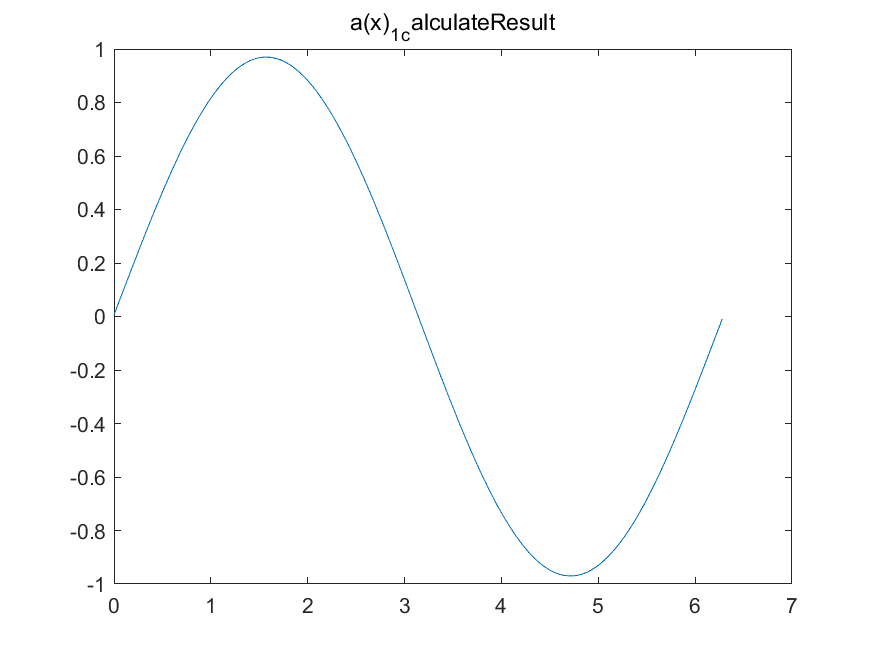
\includegraphics[height=2in, width=2in]{fig/a(x)_1_calculateResult.png}
  %\caption{fig1}
  \end{minipage}%
  }%
  \subfigure[精确解]{
  \begin{minipage}[t]{0.3\linewidth}
  \centering
  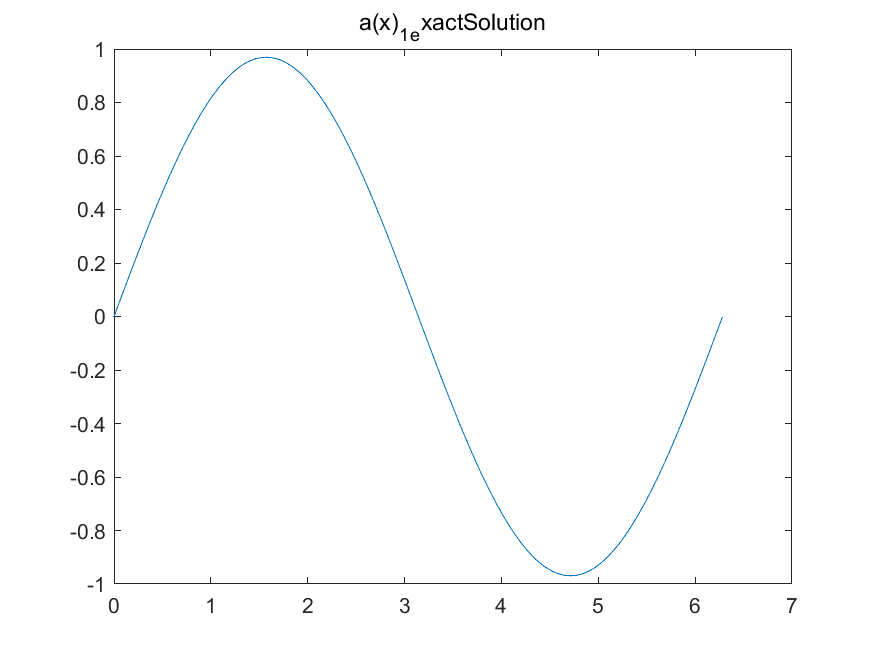
\includegraphics[height=2in, width=2in]{fig/a(x)_1_exactSolution.png}
  %\caption{fig1}
  \end{minipage}%
  }%
\end{figure}

图1.2取$a(x) = cos(x), f(x) = sin(x)$, 可知精确解为$e^{-2t cos(x)} sin(x)$. 
计算结果数值exploded.
\begin{figure}[!htbp]
  \caption{initial function 2}
  \centering
  \subfigure[数值计算结果]{
  \begin{minipage}[t]{0.3\linewidth}
  \centering
  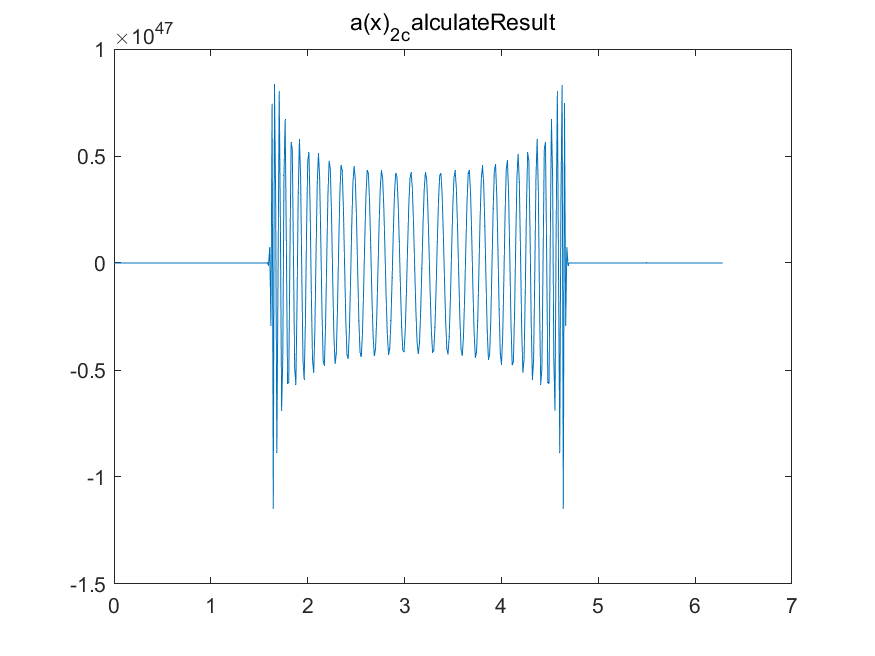
\includegraphics[height=2in, width=2in]{fig/a(x)_2_calculateResult.png}
  %\caption{fig1}
  \end{minipage}%
  }%
  \subfigure[精确解]{
  \begin{minipage}[t]{0.3\linewidth}
  \centering
  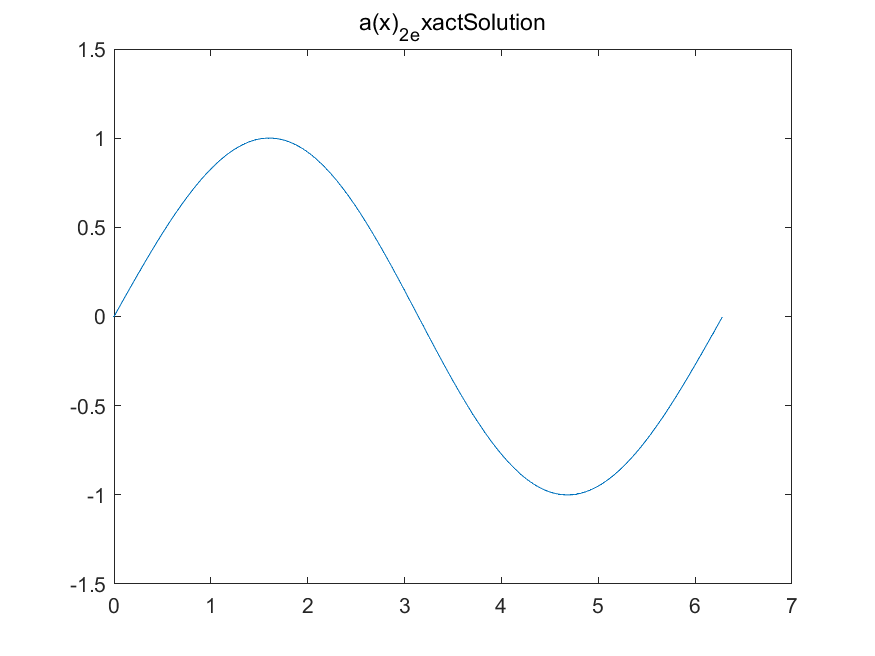
\includegraphics[height=2in, width=2in]{fig/a(x)_2_exactSolution.png}
  %\caption{fig1}
  \end{minipage}%
  }%
\end{figure}
